\documentclass{article}
\usepackage{tempora}
\usepackage{indentfirst}
\usepackage{tabularx}
\usepackage{caption}
\usepackage{graphicx}
\usepackage{longtable}
\usepackage{tabularx}
\usepackage{amsmath}
\usepackage{amsfonts}
\usepackage{floatrow}
\floatsetup[table]{capposition=top}
\makeatletter
\renewcommand*\l@section{\@dottedtocline{1}{1.5em}{2.3em}}
\makeatother
\graphicspath{ {./images/} }
\usepackage{float}
\usepackage[english, russian]{babel}

% Ответ должен быть из 2-3х абзацев по 3-4 предложения в каждом
% annakd16@mail.ru - подготовленный документ отправлять сюда
% Дьячук Анна Константиновна

% Описание системы
% 1. Какую систему Вы изучаете в Вашей диссертационной работе? Что является объектом исследования.
% 2. Каково назначение Вашей системы?
% 3. Какова цель исследования системы? Где она может быть использована?
% 4. Частью какой надсистемы является изучаемая система?
% 5. Из каких подсистем состоит система?
% 6. Какие задачи решают подсистемы в составе Вашей системы?
% 7. Сформулируйте кратко сценарий функционирования системы.
% 8. Какие факторы внешней среды Вы учитываете при анализе функционирования системы?
% 9. Какой информацией о факторах внешней среды Вы располагаете (детерминированные, случайные, интервально неопределенные, активное противодействие «противника» или конкурента)?
% 10. Какие показатели эффективности системы в целом и ее подсистем Вы рассматриваете?
% 11. Как в этих показателях учитывается информация о внешней среде?
% 12. Какое множество альтернатив системы (дискретное, непрерывное, дискретно–непрерывное) Вы рассматриваете?
% 13. Назовите основные структуры и параметры, характеризующие рассматриваемое Вами множество альтернатив системы.
% 14. При каких ограничениях на значения непрерывных параметров системы решается задача?
% 15. Составьте функциональную схему и опишите функциональные связи между подсистемами в составе системы, а также между подсистемами и внешней средой, которые Вы предполагаете учитывать при разработке математической модели системы.
% 16. Какую систему (или системы) Вы готовы рассматривать как актуальный прототип по отношению к системе, рассматриваемой в Вашей работе?
% 17. Какую задачу – анализа или синтеза системы – Вы решаете? Как решаемая задача связана с целью Вашего исследования?
% 18. Укажите тип математической модели (аналитическая, основанная на использовании физических законов и/или теории, имитационная, эмпирическая), которую Вы будете использовать для решения задачи анализа системы.
% 19. Охарактеризуйте кратко особенности разрабатываемой Вами модели системы.
% 20. В каком состоянии находится разработка модели в настоящее время?
% 21. В какой среде программирования Вы реализуете модель системы?
% 22. Если в работе решается задача синтеза системы, то какой алгоритм оптимизации альтернативы системы Вы используете или предполагаете использовать?
% 23. Если при синтезе системы рассматриваются несколько показателей ее эффективности, то как решается задача оптимизации системы по векторному критерию?
% 24. Какие новые научные и/или практические результаты Вы уже получили (или предполагаете получить) в Вашем исследовании?
% 25. Есть ли у Вас публикации по работе? Выступали ли Вы на научных конференциях по теме Вашей диссертации? Перечислите публикации, укажите место выступления (выступлений).

\begin{document}
    \begin{center}
\textbf{МИНИСТЕРСТВО ОБРАЗОВАНИЯ И НАУКИ РФ}\\[4\baselineskip]
\textbf{Федеральное государственное бюджетное образовательное учреждение высшего образования «Московский авиационный институт (национальный исследовательский университет)»}\\[4\baselineskip]
Институт № 6 «Аэрокосмический» \\[1\baselineskip]
Кафедра 604 «Системный анализ и управление»\\[4\baselineskip]
Реферат\\[2\baselineskip]
На тему: «Исследование и разработка принципов построения инструментальных средств конфигурирования в плагинных системах»\\[1\baselineskip]
По курсу: «Системный анализ»\\[4\baselineskip]
\begin{tabularx}{\textwidth}{ >{\raggedright\arraybackslash}X >{\raggedleft\arraybackslash}X }
    
Выполнил: & Шаблий А.Д. \\
Аспирант группы: & М8О-108А-23 \\
Проверила: & к.т.н. Дьячук А. К. \\
    
\end{tabularx}\\[12\baselineskip]
Москва 2024

\end{center}
    \thispagestyle{empty}
    \newpage

    \begin{enumerate}
        \item \textit{Какую систему Вы изучаете в Вашей диссертационной работе? Что является объектом исследования.}

        % Описать, что есть it
        % В it есть программные средства
        % Программные средства могут быть в виде плагинной системы

        Следуя своей диссертационной работе сложной технической системой я называю архитектуру инструментального средства конфигурирования, выполненного в виде набора плагинов. Будучи интегрированными в плагинную среду, они ее дополнят и конечный объем функционала, доступный пользователю, будет перерасчитан. Конечный объем функционала определяется суммарным объемом функционала каждого установленного в среду плагина.

        \item \textit{Каково назначение Вашей системы?}

        Архитектура предназначена для выработки правил, методов и шаблонов при разработке инструментального средства конфигурирования. 


        \item \textit{Какова цель исследования системы? Где она может быть использована?}

        Целью исследования архитектуры программного средства как сложной технической системы является формирование паттернов к ее построению, используя которые, компания-производитель снизит затраты на постпродажное обслуживание поставки программного средства, исключая неконтролируемый рост затрат на его разработку.

        Использование предполагается для решения следующей задачи:
        предположим, что по составленному техническому заданию был реализован некоторый функционал, который для возможности поставки в плагинную среду сгруппирован по плагинам. Потенциальный заказчик потребовал не весь реализованный объем, а только его часть.

        В этом случае определяется объем функционала потребный заказчику и сбор функциональных зависимостей, без которых потребный функционал не может быть поставлен.

        Результирующий объем функционала поставляется заказчику. Задача заключается в минимизации объема непотребного заказчику функционала в поставке.

        \item \textit{Частью какой надсистемы является изучаемая система?}

        Для архитектуры программного средства надсистемой является жизненный цикл программного обеспечения. Начиная от получения сформированных требований к программному средству в виде технического задания на разработку и заканчивая формированием поставки, в которую входят потребные заказчику требования.

        \item \textit{Из каких подсистем состоит система?}

        Подсистемами для архитектуры программного средства являются:
        \begin{enumerate}
            \item требования к программному обеспечению;
            \item файлы исходного кода;
            \item плагины.
        \end{enumerate}

        \item \textit{Какие задачи решают подсистемы в составе Вашей системы?}

        В требованиях к программному обеспечению описаны функциональные возможности программного средства.

        В файлах исходного кода описана реализация требований к программному обеспечению на языке программирования.

        Плагины содержат файлы исходного кода и обеспечивают их выполнение в плагинной среде.

        \item \textit{Сформулируйте кратко сценарий функционирования системы.}

        Для определения объема функционала, включенного в поставку, предполагается следующий сценарий:
        \begin{enumerate}
            \item заказчик назначает потребный объем функционала;
            \item определяется соответствующий объем потребных требований;
            \item определяются файлы исходного кода, которые реализуют потребные требования;
            \item определяются плагины, которые содержат вышеуказанные файлы исходного кода;
            \item формируется суммарная выборка файлов исходного кода, которые включены в вышеуказанные плагины;
            \item формируется суммарная выборка требований, которые реализуются в таких файлах исходного кода и делается вывод о составе поставки.
        \end{enumerate}

        \item \textit{Какие факторы внешней среды Вы учитываете при анализе функционирования системы?}

        К факторам внешней среды относятся:
        \begin{enumerate}
            \item изначальный перечень требований технического задания на разработку;
            \item потребный заказчику функционал.
        \end{enumerate}

        \item \textit{Какой информацией о факторах внешней среды Вы располагаете (детерминированные, случайные, интервально неопределенные, активное противодействие «противника» или конкурента)?}

        Изначальный перечень требований технического задания задан изначально. Изменение его состава согласуется со всеми участниками жизненного цикла программного обеспечения и актуальные данные о нем известен потенциальному заказику.

        Потребный заказчику функционал транслируется в требования. Общий перечень требований описан в техническом задании на разработку. Таким образом потребные требования не могут выходить за рамки множества требований описанных в техническом задании.

        \item \textit{Какие показатели эффективности системы в целом и ее подсистем Вы рассматриваете?}

        К показателям эффективности относятся:
        \begin{enumerate}
            \item возможность формирования различных комплектаций поставки программного средства;
            \item объем кодовой базы проекта;
            \item отношение числа невостребованных требований к общему числу реализованных требований в поставке.
        \end{enumerate}

        \item \textit{Как в этих показателях учитывается информация о внешней среде?}

        Благодаря возможности формирования различных комплектаций достигается уменьшение коэффициента бесполезности при 

        \begin{center}
        $
            \begin{cases}
                R^1_{n} \not = R^2_{n}\\
                |R^1_{n}| = |R^2_{n}|
            \end{cases}
        $
        \end{center}

        где: $R^1_{d}$ и $R^2_{d}$ - множества востребованных требований в рамках разных поставок

        \begin{center}
            $F_{p} = 
            \begin{cases}
                1 \quad \text{если условие выполняется}\\
                0 \quad \text{если условие не выполняется}
            \end{cases}
            $
        \end{center}

        где: $F_{p}$ - возможность формирования различных комплектаций 

        Объем кодовой базы влияет на стоимость разработки и поддержки проекта. Чем он больше - тем дороже разработка и поддержка. Объем кодовой базы зависит от двух факторов:
        \begin{enumerate}
            \item чем больше требований технического задания - тем больше объем кодовой базы;
            \item количество ограничений на наличие функциональных зависимостей. Чем больше ограничений, тем более сложные связи. Чем сложнее связи - тем больше объем кодовой базы. Сложность связей увеличивается, если элементы цепочки зависимостей находятся в разных плагинах.
        \end{enumerate}

        \begin{center}
            $V_{c} = 
            \begin{cases}
                1 & \quad \text{если } |P^*| = 1\\
                2 & \quad \text{если } |C^*| \gg |P^*|\\
                3 & \quad \text{если } |C^*| \not \gg |P^*|
            \end{cases}
            $,
        \end{center}

        где: $V_{c}$ - объем кодовой базы\\
        $P^*$ - множество плагинов\\
        $C^*$ - множество файлов исходного кода

        В формируюемую поставку включаются как потребные требования, так и невостребованные. Исходя из потребных заказчику требований формируется цена поставки, в которую включена цена на постпродажное обслуживание. Коэффициентом бесполезности характеризуется объем выполняемых работ подразделениями постпродажного обслуживания неоплаченного заказчиком и выполняемом за счет компании-поставщика.

        \begin{center}
            $K_{f} = \frac{|R^*_{un}|}{|R^*_{d}|}$,
        \end{center}

        где: $K_{f}$ - коэффициент бесполезности\\
        $R^*_{un}$ - множество требований невостребованных заказчиком в рамках поставки\\
        $R^*_{d}$ - множество требований реализованных в рамках поставки

        \item \textit{Какое множество альтернатив системы (дискретное, непрерывное, дискретно–непрерывное) Вы рассматриваете?}

        Рассматриваются две альтернативы системе:
        \begin{enumerate}
            \item построение по схеме <<1 требование - 1 плагин>>;
            \item построение по схеме <<все требования - 1 плагин>>.
        \end{enumerate}

        Для альтернативы <<1 требование - 1 плагин>> характерно:
        \begin{enumerate}
            \item один файл исходного кода не может реализовывать более одного требования;
            \item файл исходного кода не может иметь зависимость на другой файл исходного кода если они реализуют разные требования;
            \item плагин не может включать файлы исходного кода, которые реализуют разные требования.
        \end{enumerate}

        Для альтернативы <<все требования - 1 плагин>> характерно:
        \begin{enumerate}
            \item нет ограничений на число требований, которое реализует один файл исходного кода;
            \item нет ограничений на число и характер зависимостей между файлами исходного кода;
            \item в проекте один плагин, который включает все файлы исходного кода.
        \end{enumerate}

        \item \textit{Назовите основные структуры и параметры, характеризующие рассматриваемое Вами множество альтернатив системы.}

        Для альтернативы <<1 требование - 1 плагин>> характерно:
        \begin{enumerate}
            \item $F_{p} = 1$
            \item $V_{c} = 3$;
            \item $K_{f} = 0$.
        \end{enumerate}

        Здесь объем кодовой базы максимален из-за невозможности переиспользовать код, который участвует в реализации других требований. Появляется необходимость в создании большого числа сущностей в проекте, что приводит к неконтролируемому росту стоимости разработки и сопровождения.

        Коэффициент бесполезности минимален и равен 0. Данная схема гарантирует, что в формируемую поставку не войдет функционал, реализующий невостребованные требования.

        Для альтернативы <<все требования - 1 плагин>> характерно:
        \begin{enumerate}
            \item $F_{p} = 0$
            \item $V_{c} = 1$;
            \item $K_{f} \approx 1$.
        \end{enumerate}

        Здесь объем кодовой базы минимален. Нет искусстенных ограничений на построение кода, что существенно снижает стоимость разработки и поддержки проекта.

        Однако коэффициент бесполезности принимает максимальное значение. Это говорит о том, что практически вся работа служб постпродажного обслуживания производится за счет компании-поставщика.



        \item \textit{При каких ограничениях на значения непрерывных параметров системы решается задача?}

        Уменьшение числа невостребованных требований в формируемой поставке целесообразно при выполнении условия: 
        \begin{center}
            $|R^*_{n}| \ll |R^*|$,
        \end{center}

        где: $R^*_{n}$ - множество требований потребных заказчиком \\
        $R^*$ - множество требований технического задания

        Альтернативу <<1 требование - 1 плагин>> целесообразно применять при $|R^*| \not \gg 0$.

        Альтернативу <<все требования - 1 плагин>> целесообразно применять при $|R^*_{n}| \approx |R^*|$.

        \item \textit{Составьте функциональную схему и опишите функциональные связи между подсистемами в составе системы, а также между подсистемами и внешней средой, которые Вы предполагаете учитывать при разработке математической модели системы.}

        Функциональные связи между подсистемами следующие:
        \begin{enumerate}
            \item одно требование может быть реализовано в одном или нескольких файлах исходного кода;
            \item один файл исходного кода может реализовывать одно или несколько требований;
            \item один файл исходного кода не может быть включен в несколько плагинов;
            \item файлы исходного кода могут иметь зависимости друг на друга, в том числе и циклические;
            \item плагины так же имеют друг на друга зависимости: если первый плагин содержит файл имеющий зависимость на файл из второго плагина, то первый плагин имеет зависимость на второй плагин;
            \item циклические зависимости между плагинами запрещены.
        \end{enumerate}

        Функциональная схема связей подсистем друг с другом приведена на рисунке \ref{fig:graph}.

        \begin{figure}[H]
            \centering
            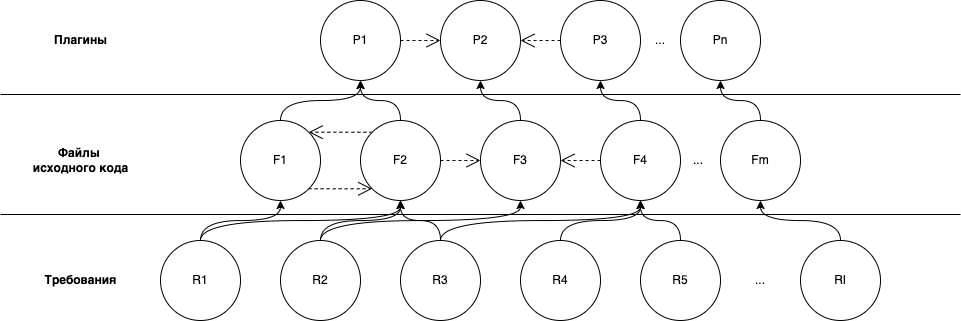
\includegraphics[width=1\textwidth]{graph}
            \caption{Схема связей подсистем}
            \label{fig:graph}
        \end{figure}

        Функциональная схема связи системы с внешней средой приведена на рисунке \ref{fig:life_circle}.

        \begin{figure}[H]
            \centering
            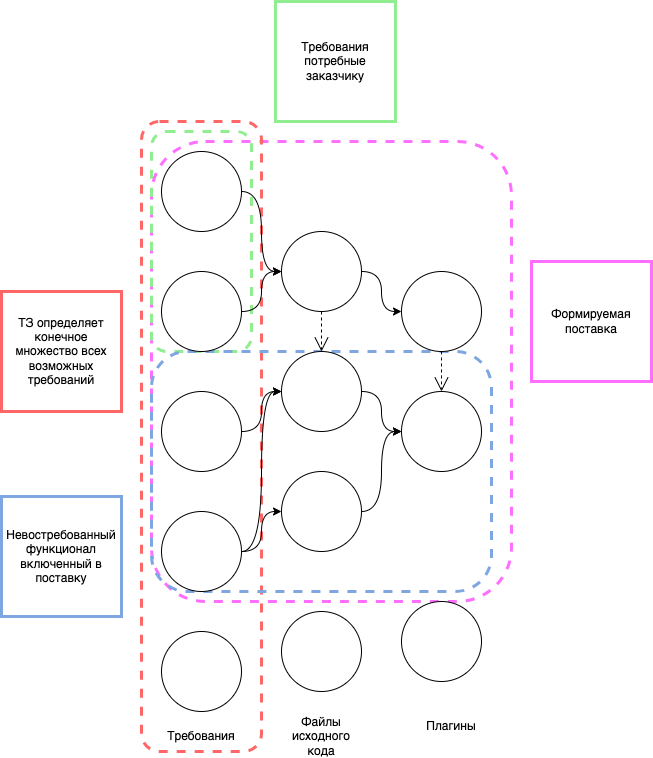
\includegraphics[width=0.8\textwidth]{life_circle}
            \caption{Связь системы и надсистемы}
            \label{fig:life_circle}
        \end{figure}

        \item \textit{Какую систему (или системы) Вы готовы рассматривать как актуальный прототип по отношению к системе, рассматриваемой в Вашей работе?}

        В качестве актуального прототипа по отношению к рассматриваемой системе я рассматриваю спецификацию OSGI. В частности ее реализацию Equinox в IDE Eclipse. Благодаря ей достигается возможность создавать приложения в виде группы наборов, использующих общие сервисы и инфраструктуру.

        \item \textit{Какую задачу – анализа или синтеза системы – Вы решаете? Как решаемая задача связана с целью Вашего исследования?}

        Я решаю задачу синтеза системы. Цель моего диссертационного исследования - разработка и формулировка правил построения инструментальных средств конфигурирования в плагинных системах. Решая задачу синтеза системы, я раскрываю тематику построения решений в плагинных средах, а именно:

        \begin{enumerate}
            \item выявление элементов предметной области;
            \item их анализ, сравнение характеристик;
            \item описание ограничений;
            \item формирование математической модели. 
        \end{enumerate}

        \item \textit{Укажите тип математической модели (аналитическая, основанная на использовании физических законов и/или теории, имитационная, эмпирическая), которую Вы будете использовать для решения задачи анализа системы.}

        Я использую графовую модель.

        \item \textit{Охарактеризуйте кратко особенности разрабатываемой Вами модели системы.}

        Вершинами являются элементы подсистем:
        \begin{enumerate}
            \item требования;
            \item файлы исходного кода;
            \item плагины.
        \end{enumerate}

        Ребрами являются функциональные связи:
        \begin{enumerate}
            \item трассируемость требований к программному обеспечению на файлы исходного кода;
            \item распределение файлов исходного кода по плагинам;
            \item зависимости между файлами исходного кода;
            \item зависимости между плагинами.
        \end{enumerate}

        \item \textit{В каком состоянии находится разработка модели в настоящее время?}

        В настоящее время разработан модуль, описывающий работу двух слоев:
        \begin{enumerate}
            \item требований к программному обеспечению;
            \item файлов исходного кода.
        \end{enumerate}

        \item \textit{В какой среде программирования Вы реализуете модель системы?}

        Я реализую модель системы в среде программирования Java.

        \item \textit{Если в работе решается задача синтеза системы, то какой алгоритм оптимизации альтернативы системы Вы используете или предполагаете использовать?}

        В своей дальнейшей работе по реализации модели я предполагаю использовать следующие алгоритмы оптимизации:
        \begin{enumerate}
            \item генетический алгоритм;
            \item PageRank;
            \item случайный лес;
        \end{enumerate}

        \item \textit{Если при синтезе системы рассматриваются несколько показателей ее эффективности, то как решается задача оптимизации системы по векторному критерию?}

        Ожидается, что выявленная оптимальная декомпозиция функционала по плагинам обеспечит следующие показатели эффективности:
        \begin{enumerate}
            \item $F_{p} = 1$;
            \item $V_{c} = 2$;
            \item $0 \leq K_{f} < 1$.
        \end{enumerate}

        Сравнение показателей эффективности приведено в таблице \ref{tab:difference}.

        \begin{table}[H]
        \begin{tabularx}{\textwidth}{ |>{\center\arraybackslash}X|>{\center\arraybackslash}X|>{\center\arraybackslash}X|>{\center\arraybackslash}X| }
        
        \hline
        & $F_{p}$ & $V_{c}$ & $K_{f}$ \\
        \hline
        <<1 требование - 1 плагин>> & 1 & 3 & 0 \\
        \hline
        <<все требования - 1 плагин>> & 0 & 1 & $\approx 1$ \\
        \hline
        предлагаемое решение & 1 & 2 & $\{x \in \mathbb{R}: 0 \leq x < 1\}$ \\
        \hline
            
        \end{tabularx}
        \caption{Сравнение показателей эффективности}
        \label{tab:difference}
        \end{table}

        Необходимо, чтобы $F_{p}$ решения был равен 1. По этому условию <<все требования - 1 плагин>> не подходит. Из оставшихся вариантов выбирая между минимизацией $V_{c}$ и $K_{f}$ отдается предпочтение минимизации $V_{c}$.

        \item \textit{Какие новые научные и/или практические результаты Вы уже получили (или предполагаете получить) в Вашем исследовании?}

        Разработанный модуль применяется для проведения экспериментов по разрешению циклических зависимостей между файлами исходного кода. Произведено исследование зависимости времени работы решения от используемых в программе реализаций Java-коллекций.

        \item \textit{Есть ли у Вас публикации по работе? Выступали ли Вы на научных конференциях по теме Вашей диссертации? Перечислите публикации, укажите место выступления (выступлений).}

        На конференции в МГТУ им. Баумана я в своем докладе «Исследование правил построения конфигуратора ARINC 653 спецификации в IDE Eclipse» показал результаты применения сформулированной модели для решения задачи путем разбиения файлов исходного кода по плагинам по частотам вызова функций. В качестве результата продемонстрировал снижение невостребованного функционала до 10\% при различных запросах состава требований.

        На конференции в Воронеже в ВУНЦ ВВС «ВВА имени профессора Н.Е. Жуковского и Ю.А. Гагарина» в своем докладе «Реализация инструментального средства конфигурирования компонентов БРЭО» показал актуальность применения плагинных систем для решения задач в авиационной сфере.

        Подготовил выступление на конференции, организуемой Союзом Машиностроителей России. В качестве материала выступления мною предоставлено средство интеллектуального конфигурирования системы определения состояния воздушного судна. В этой работе я сформировал среду конфигурирования, которая независимо подключается к базе данных и заполняет ее конфигурационными параметрами и их значениями с целью дальнейшей их обработки непосредственно в самой системе.

        Подготовлена публикация ВАК, в которой описан алгоритм разрешения циклических зависимостей графовой модели трассируемости требований к ПО на файлы исходного кода. Работа передана в редакцию ИПМ им. М.В.Келдыша РАН.

    \end{enumerate}

\end{document}